\documentclass{article}
\usepackage{amsmath}
\usepackage{amsfonts}
\usepackage{bm}
\usepackage{graphicx}
\usepackage{float}
\usepackage{subfigure}
\usepackage{enumitem}
\usepackage{ctex}
\usepackage{multirow}

\renewcommand{\figurename}{Figure}


\begin{document}
\begin{titlepage}
\vspace*{\fill}
\begin{center}
\huge Statistical Learning \\Computer Homework\\ 109064509 楊暐之
\end{center}
\vspace{\fill}
\end{titlepage}


\begin{enumerate}
{ \Large \bf \item \  }\\
	\begin{enumerate}
	
	%Problem 1(a)
	{ \large \bf \item \  }\\
		\begin{tabular}{|c|c|c|c|c|}
		\hline
						&	Coefficient	&	Std. Error	&	t-statistic & p-value\\
		\hline
		\multirow{2}*{\shortstack{$\beta_0$\\(intercept)}}	&	\multirow{2}*{-0.1785}	&	\multirow{2}*{0.1824}	&	\multirow{2}*{-0.9783}	&	\multirow{2}*{0.1647}\\
		&&&&\\
		\hline
		$X_1$			&	0.0853	&	0.0560	&	1.5242	&	0.0647	\\
		\hline
		$X_2$			&	0.0045	&	0.0113	&	0.4015	&	0.3443	\\
		\hline  
		$X_3$			&	-0.0907	&	0.4654	&	-0.1949	&	0.4229	\\
		\hline  	
		$X_4$			&	-0.0578	&	0.1118	&	-0.5173	&	0.3028	\\
		\hline 
		$X_5$			&	0.1411	&	0.2354	&	0.5993	&	0.2749	\\
		\hline 
		$X_6$			&	0.0330	&	0.0060	&	5.4952	&	 $<0.0001$	\\
		\hline 
		\end{tabular}\\[1cm]		
	%Problem 1(b)
	{ \large \bf \item \  }\\
		\begin{tabular}{|c|c|c|c|c|}
		\hline
						&	Coefficient	&	Std. Error	&	t-statistic & p-value\\
		\hline
		$X_1$			&	0.0843	&	0.0542	&	1.5553	&	0.0609	\\
		\hline
		$X_6$			&	0.0344	&	0.0053	&	6.4921	&	$<0.0001$	\\
		\hline 
		\end{tabular}\\[1cm]
		To compare with the result in (c), more precisely, the coefficient of $X_1,X_6$ are 0.08428384 0.03444787, resp.\\
		Note that the two predictors that yields the smallest RSS are also the two predictors with smalles p-value in (a)
		
	\newpage
	
	%Problem 1(c)
	{ \large \bf \item \  }\\
		\begin{tabular}{|c|c|}
		\hline
		$\lambda=10^{-1.5}$	&	Coefficient	\\
		\hline
		$X_1$			&	0.0843	\\
		\hline
		$X_6$			&	0.0344	\\
		\hline 
		\end{tabular}\\[1cm]
		To compare with the result in (b), more precisely, the coefficient of $X_1,X_6$ are 0.08428384 0.03444787, resp.\\
		I use all predictors to caculate $\mathrm{CV}_{(5)}$ for each $\lambda$ and then choose $\lambda^*$ as
		\begin{equation*}
		\lambda^*=\arg\min\limits_\lambda \mathrm{CV}_{(5)}
		\end{equation*}
		Then, find the predictors that yield the smallest RSS with $\lambda=\lambda^*$
		
		\begin{figure}[H]
		\centering
		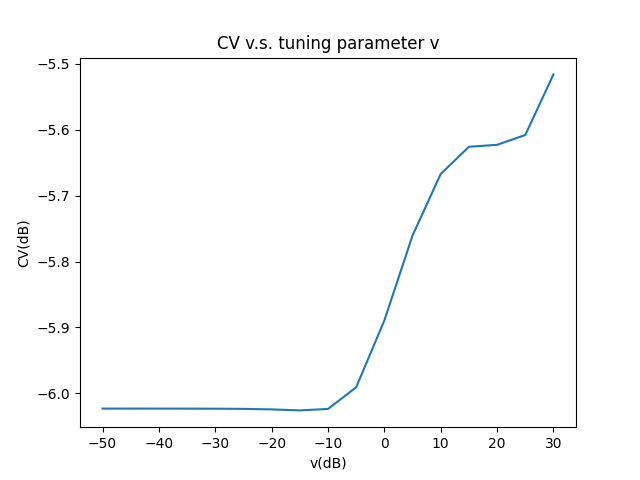
\includegraphics[width=\textwidth]{CV_vs_lambda}
		\end{figure}
	\end{enumerate}

\newpage

{ \Large \bf \item \  }\\
	\begin{enumerate}
	{ \large \bf \item \  }\\
		Initial conditions : \\
		step size : 0.1\\
		$\bf\beta$ : $\bm\vec{0}$\\
		Termination condition : \\
		$\nabla J(\beta)\leq10000$\\
		\begin{tabular}{|c|c|c|c|c|}
		\hline
						&			&\multicolumn{3}{c|}{True label}\\
						&			&\multicolumn{2}{c|}{1\quad\qquad 2}&Total\\
		\hline
		\multirow{2}*{\shortstack{Predicted \\label}}	&	1	&	618	&	23	&	641\\
						&	2		&	406		&	1001	&	1407	\\
		\cline{2-5}
						&	Total	&	1024	&	1024	&	2048	\\
		\hline 
		\end{tabular}\\[0.2cm]
		error rate of label 1 is 39.6\%\\
		error rate of label 2 is 2.2\%\\
		average error rate is 20.9\%\\

		Change termination condition to \\
		$\nabla J(\beta)\leq100$\\	
		\begin{tabular}{|c|c|c|c|c|}
		\hline
						&			&\multicolumn{3}{c|}{True label}\\
						&			&\multicolumn{2}{c|}{1\quad\qquad 2}&Total\\
		\hline
		\multirow{2}*{\shortstack{Predicted \\label}}	&	1	&	639	&	35	&	674\\
						&	2		&	385		&	989 &	1374	\\
		\cline{2-5}
						&	Total	&	1024	&	1024	&	2048	\\
		\hline 
		\end{tabular}\\[0.2cm]
		error  rate of label 1 is 37.6\%\\
		error rate of label 2 is 3.4\%\\
		average error rate is 20.5\%\\[0.2cm]
		The performance is only slightly improved by changing the termination condition, and it recognizes label 2 much more accurately than label 1. It is possible that label 1 is similar to label 2 , but the converse is not true for the training results in some degree.\\
	{ \large \bf \item \  }\\
	\end{enumerate}
\end{enumerate}

\end{document}